\documentclass[UTF8,aspectratio=169]{ctexbeamer}
\usetheme{Madrid}
\usecolortheme{whale}
\usefonttheme{professionalfonts}

\catcode`。=\active
\def。{.}

\usepackage{graphicx}
\graphicspath{{fig/}}
\usepackage{subfigure}

\usepackage{mathtools}
%\usepackage{amsmath,amssymb,amsthm}
\usepackage{pifont}
\usepackage{array}
\usepackage{booktabs}

\newenvironment<>{question}[1][]{
        \begin{exampleblock}#2{问题}}{\end{exampleblock}}
\newenvironment<>{answer}[1][]{
        \begin{alertblock}#2{答案}}{\end{alertblock}}

\usepackage{tikz}
\newcommand\tikzmark[1]{
        \tikz[overlay,remember picture] \node[coordinate] (#1) {};
}


\author{王介哲}
\institute{优才教育}
\title{数学分班打卡课 第四周(2)}
\date{2018年5月}

\begin{document}

\frame{\titlepage}

\begin{frame}
\begin{question}
        \qquad 计算:\(1\dfrac{4}{17} \times \left(2\dfrac{2}{3} - 0.75\right) + 15\dfrac{1}{12} \div \dfrac{17}{21}\)。
\end{question} \pause
\begin{answer} \pause
        \[
        \begin{aligned}
                \text{原式} &= \frac{21}{17} \pause \times \left(\frac{8}{3} - \frac{3}{4}\right) \pause
                                          + 15 \times \frac{21}{17} + \frac{1}{12} \times \frac{21}{17} \\ \pause
                &= \frac{21}{17} \times \left(\frac{8}{3} - \frac{3}{4} + 15 + \frac{1}{12}\right) \\ \pause
                &= \frac{21}{17} \times \left(\frac{23}{12} + 15 + \frac{1}{12}\right) \\ \pause
                &= \frac{21}{17} \times \left(2 + 15\right) \\ \pause
                &= \frac{21}{17} \times 17 \\ \pause
                &= 21
        \end{aligned}
        \]
\end{answer}
\end{frame}

\begin{frame}
\begin{question}
        甲容器中有纯酒精 $10$ 升,乙容器中有水 $16$ 升,第一次将甲容器中的一部分纯酒精倒入乙容器,使酒精与水混合;第二次将乙容器中一部分混合液倒入甲容器,这样甲容器中纯酒精含量为 $50\%$,乙容器中纯酒精含量为 $20\%$。那么,第二次从乙容器倒入甲容器的混合液是多少升?
\end{question} \pause
\begin{block}{分析} \pause
        \begin{itemize}
                \item 两容器中溶液总量一定,为 $26$ 升;酒精总量也一定,为 $10$ 升 \pause
                \item 第一次操作前后,两容器中水的量不变 \pause
                \item 第二次操作前后,乙容器中酒精的浓度不变
        \end{itemize}
\end{block}
\end{frame}

\begin{frame}
        \begin{answer}
                设最终甲容器中有 $x$ 升溶液,乙容器中有 $y$ 升溶液。\\ \pause
                由题知,
                \[
                \begin{dcases}
                x + y = 26 \\
                0.5 x + 0.2 y = 10
                \end{dcases}
                \] \pause
                解得
                \(
                \begin{dcases}
                x = 16 \\
                y = 10
                \end{dcases}
                \)。
        \end{answer}

\end{frame}

\begin{frame}
        \begin{answer}
                \renewcommand\arraystretch{1.5}
                \begin{table}[h]
                        \caption{甲、乙两容器中溶液变化情况(酒精:水/总容量)}
                        \vspace{1ex}
                        \begin{tabular}{m{2cm}<{\centering} m{2cm}<{\centering}}
                                \toprule
                                甲 & 乙 \\
                                \midrule
                                10:0/10 \tikzmark{1 start} &  \tikzmark{1 end} 0:16/16 \\
                                \ding{88}:0/\ding{88} \tikzmark{2 start} & \tikzmark{2 end} \only<1-3>{\ding{115}}\only<4->{\alert{4}}:16/\only<1-4>{\ding{110}}\only<5->{\alert{20}} \\
                                8:8/16 & 2:8/10 \\
                                \bottomrule
                        \end{tabular}
                \end{table} \pause
                \begin{tikzpicture}[overlay, remember picture]
                		\draw[thick, blue,->] (1 start) to [bend left](1 end);
                \end{tikzpicture} \pause
                \begin{tikzpicture}[overlay, remember picture]
                		\draw[thick, blue, <-] (2 start) -- node[below]{?:8/??} (2 end);
                \end{tikzpicture}
                \vspace{1ex}
                \uncover<6->{\qquad 故第二次从乙倒入甲 $20 - 10 = 10$ 升。}
        \end{answer}
\end{frame}

\begin{frame}
\begin{question}
        \begin{columns}[c]
        \begin{column}{0.6\textwidth}
                如图,长方形的长是 $8$,宽是 $6$,$A$ 和 $B$ 是宽的中心,则长方形内阴影部分的面积为\underline{\qquad\qquad}.
        \end{column}
        \begin{column}{0.2\textwidth}
                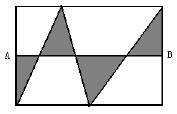
\includegraphics[width=\textwidth]{3.jpg}
        \end{column}
        \end{columns}
\end{question} \pause
\begin{answer} \pause
        \[8 \times 3 \div 2 = 12\]
\end{answer}
\end{frame}

\end{document}
